% Kompilacja (z katalogu docs/presentations):  latexmk -pdf prezentacja.tex
\documentclass[aspectratio=169,10pt]{beamer}

\usepackage[T1]{fontenc}
\usepackage[utf8]{inputenc}
\usepackage[polish]{babel}
\usepackage{lmodern}
\usepackage{tgheros}
\renewcommand{\familydefault}{\sfdefault}
\usepackage{graphicx}
\usepackage{booktabs}
\usepackage{array}
\usepackage{tikz}
\usetikzlibrary{positioning,arrows.meta,calc}
\usepackage{pgfplots}
\pgfplotsset{compat=1.18,
  square legend/.style={legend image code/.code={\fill[##1] (0cm,-0.1cm) rectangle (0.25cm,0.15cm);}}}
\usepackage[most]{tcolorbox}
\usepackage{fontawesome5}

% ============================================================
% Kolory
% ============================================================
\definecolor{ink}{HTML}{1F2328}       % tekst główny
\definecolor{muted}{HTML}{646B75}     % tekst drugorzędny
\definecolor{faint}{HTML}{D7D9DD}     % linie, siatka
\definecolor{paper}{HTML}{FAFAF8}     % tło slajdów
\definecolor{card}{HTML}{FFFFFF}      % tło kart
\definecolor{night}{HTML}{14161B}     % tło slajdu tytułowego
\definecolor{accent}{HTML}{D9480F}    % akcent (pomarańczowo-czerwony)
\definecolor{accentsoft}{HTML}{FBE6DC}
\definecolor{control}{HTML}{3F6FB5}     % druga seria na wykresach (agent bez strzelania)

% ============================================================
% Wygląd beamera
% ============================================================
\setbeamercolor{background canvas}{bg=paper}
\setbeamercolor{normal text}{fg=ink}
\setbeamercolor{frametitle}{fg=ink}
\setbeamercolor{structure}{fg=accent}
\setbeamercolor{alerted text}{fg=accent}
\setbeamerfont{frametitle}{size=\Large,series=\bfseries}
\setbeamertemplate{navigation symbols}{}
\setbeamertemplate{itemize items}{\color{accent}\small$\blacktriangleright$}
\setbeamertemplate{itemize subitem}{\color{muted}\small--}
\setbeamersize{text margin left=12mm,text margin right=12mm}

% Tytuł slajdu: numer sekcji w kolorze akcentu + tytuł
\newcommand{\slidenum}{}
\setbeamertemplate{frametitle}{%
  \vspace*{5mm}%
  \ifx\slidenum\empty\else
    {\color{accent}\slidenum}\hspace{3mm}{\color{faint}|}\hspace{3mm}%
  \fi
  \insertframetitle\par\vspace{-1mm}%
}

% Stopka: autorzy po lewej, numer slajdu po prawej, cienki pasek postępu
\setbeamertemplate{footline}{%
  \ifnum\insertframenumber>1
  \begin{tikzpicture}[remember picture,overlay]
    \fill[faint] (current page.south west) rectangle ([yshift=1.2pt]current page.south east);
    \fill[accent] (current page.south west) rectangle
      ([yshift=1.2pt]$(current page.south west)!{\insertframenumber/\inserttotalframenumber}!(current page.south east)$);
    \node[anchor=south west,font=\scriptsize,text=muted,inner sep=0]
      at ([xshift=12mm,yshift=4mm]current page.south west) {\insertshortauthor\ \ \textbullet\ \ \insertshorttitle};
    \node[anchor=south east,font=\scriptsize\bfseries,text=muted,inner sep=0]
      at ([xshift=-12mm,yshift=4mm]current page.south east)
      {\insertframenumber\,/\,\inserttotalframenumber};
  \end{tikzpicture}%
  \fi
}

% Karta z ikoną i nagłówkiem
\newtcolorbox{infocard}[2]{%
  enhanced, colback=card, colframe=faint, boxrule=0.5pt, arc=2mm,
  left=3mm, right=3mm, top=2mm, bottom=2mm,
  borderline west={2pt}{0pt}{accent},
  fontupper=\footnotesize, before skip=0pt, after skip=2mm,
  title={\textcolor{accent}{#1}\hspace{2mm}\textbf{#2}},
  coltitle=ink, colbacktitle=card, attach title to upper, after title={\par\vspace{0.8mm}}}

% Duża liczba z opisem i przedziałem ufności
\newcommand{\bignum}[3]{%
  \begin{tcolorbox}[enhanced, colback=card, colframe=faint, boxrule=0.5pt, arc=2mm,
      left=3mm, right=2mm, top=1.5mm, bottom=1.5mm, borderline west={2pt}{0pt}{accent},
      before skip=0pt, after skip=2mm]
    {\fontsize{18}{20}\selectfont\bfseries #1}\par\vspace{0.5mm}
    {\footnotesize #2}\par
    {\scriptsize\color{muted} #3}
  \end{tcolorbox}}

% Obrazek z ramką i podpisem
\newcommand{\shot}[3]{%
  \begin{tikzpicture}
    \node[inner sep=0] (img) {\includegraphics[width=#1]{#2}};
    \draw[faint,line width=0.6pt,rounded corners=1mm] (img.south west) rectangle (img.north east);
  \end{tikzpicture}\par\vspace{1mm}
  {\scriptsize\color{muted}#3}}

\title{Agent RL w ViZDoom}
\subtitle{Scenariusz Deathmatch}
\author[M.\,Piechota, H.\,Sobociński]{Michał Piechota, Hubert Sobociński}
\date{}

\begin{document}

% ============================================================
% Slajd tytułowy: pełnoekranowy zrzut z gry
% ============================================================
{
\setbeamertemplate{background}{%
  \begin{tikzpicture}[remember picture,overlay]
    \node[inner sep=0] at (current page.center)
      {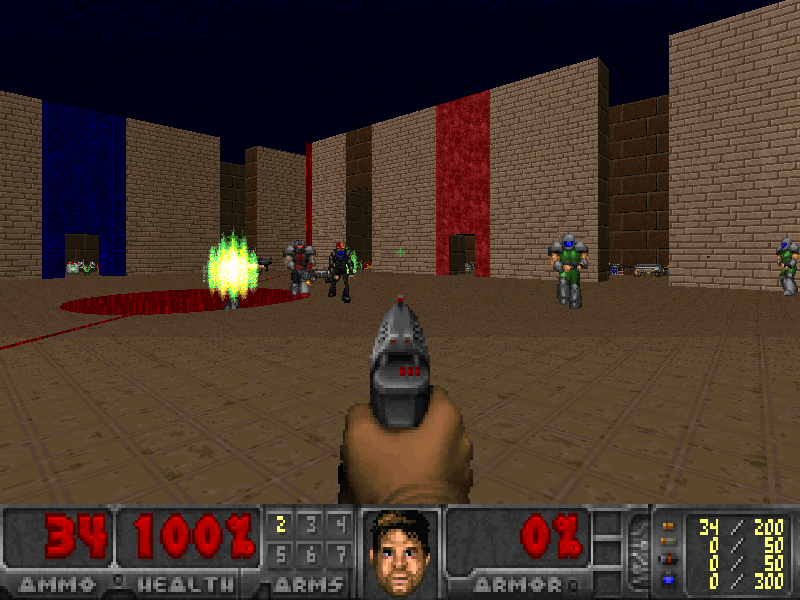
\includegraphics[width=\paperwidth,height=\paperheight,keepaspectratio=false]{img/arena.png}};
    \fill[night,opacity=0.78] (current page.south west) rectangle (current page.north east);
    \fill[night,opacity=0.9] (current page.south west) rectangle ([xshift=0.62\paperwidth]current page.north west);
  \end{tikzpicture}}
\begin{frame}[plain]
  \vspace*{10mm}
  {\color{accent}\small\bfseries\MakeUppercase{Uczenie ze wzmocnieniem}\par}
  \vspace{1.5mm}
  {\color{accent}\rule{18mm}{1.5pt}\par}
  \vspace{5mm}
  {\color{white}\fontsize{34}{38}\selectfont\bfseries Agent RL w ViZDoom\par}
  \vspace{2mm}
  {\color{white!75!night}\Large Scenariusz Deathmatch\par}
  \vspace{14mm}
  {\color{white!85!night}\normalsize Michał Piechota \quad\textbullet\quad Hubert Sobociński\par}
\end{frame}
}

% ============================================================
\renewcommand{\slidenum}{01}
\begin{frame}{Środowisko i zadanie}
  \begin{columns}[T,onlytextwidth]
    \begin{column}{0.55\textwidth}
      \begin{infocard}{\faCrosshairs}{Cel agenta}
        Zabić jak najwięcej potworów, zanim skończy się czas albo agent zginie.
        Potwory pojawiają się losowo co kilka sekund i atakują gracza.
      \end{infocard}
      \begin{infocard}{\faTrophy}{Nagroda}
        Za każde zabójstwo; wartość zależy od trudności potwora
        (np.~3 zabójstwa $\rightarrow$ 8 pkt).
      \end{infocard}
      \begin{infocard}{\faGamepad}{Akcje}
        17 przycisków: ruch, obrót, strafe, sprint, strzał, wybór broni.
        Agent wybiera \textbf{1 z 18 akcji}: brak akcji albo jeden przycisk.
      \end{infocard}
    \end{column}
    \begin{column}{0.41\textwidth}
      \vspace{1mm}
      \shot{\linewidth}{img/arena.png}{Przeciwnicy na arenie, widok z~HUD (agent dostaje obraz bez HUD)}\par
      \vspace{3mm}
      {\footnotesize
      \faFlagCheckered\hspace{1.5mm}\textbf{Koniec epizodu:} śmierć agenta
      albo limit 4200 tików ($\approx$\,2~min gry)\par}
    \end{column}
  \end{columns}
\end{frame}

% ============================================================
\renewcommand{\slidenum}{02}
\begin{frame}{Wejście dla agenta}
  \begin{columns}[T,onlytextwidth]
    \begin{column}{0.44\textwidth}
      \small
      \begin{itemize}\setlength\itemsep{2.5mm}
        \item \textbf{Wyłącznie obraz} -- ostatnia klatka gry, 3~kanały RGB
        \item Silnik renderuje \textbf{320\,$\times$\,240}; przed siecią
          skalujemy do \textbf{60\,$\times$\,45}
          i~przetwarzamy CNN-em
        \item \textbf{Frame skip = 4} -- agent decyduje co 4.~klatkę, a~na
          pominiętych powtarza ostatnią akcję. Kompromis: szybsze uczenie
          vs.~precyzja celowania
      \end{itemize}
    \end{column}
    \begin{column}{0.54\textwidth}
      \centering
      \begin{tikzpicture}[node distance=7mm]
        \node[inner sep=0] (raw) {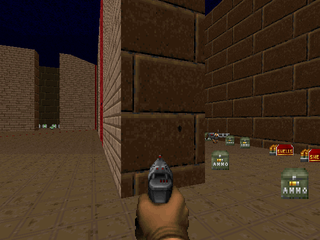
\includegraphics[width=0.43\linewidth]{img/input_320x240.png}};
        \node[inner sep=0,right=of raw] (small) {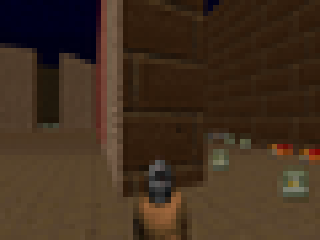
\includegraphics[width=0.43\linewidth]{img/input_60x45.png}};
        \draw[faint,line width=0.6pt] (raw.south west) rectangle (raw.north east);
        \draw[faint,line width=0.6pt] (small.south west) rectangle (small.north east);
        \draw[-{Stealth[length=2.5mm]},accent,line width=1.2pt] (raw.east) -- (small.west);
        \node[below=1.5mm of raw,font=\scriptsize,text=muted] {320\,$\times$\,240\,$\times$\,3};
        \node[below=1.5mm of small,font=\scriptsize,text=muted] {60\,$\times$\,45\,$\times$\,3};
      \end{tikzpicture}

      \vspace{5mm}
      % Oś czasu frame skip
      \begin{tikzpicture}[x=5.2mm,y=1mm]
        \foreach \i in {0,...,11} {
          \pgfmathtruncatemacro{\d}{mod(\i,4)==0}
          \ifnum\d=1
            \fill[accent] (\i,0) rectangle ++(0.8,6);
          \else
            \fill[accentsoft] (\i,0) rectangle ++(0.8,6);
          \fi
        }
        \node[anchor=north west,font=\scriptsize,text=muted] at (0,-1.5) {klatki gry};
        \fill[accent] (5.6,-5.2) rectangle ++(0.6,2.4);
        \node[anchor=west,font=\scriptsize,text=muted] at (6.3,-4) {decyzja};
        \fill[accentsoft] (9.0,-5.2) rectangle ++(0.6,2.4);
        \node[anchor=west,font=\scriptsize,text=muted] at (9.7,-4) {powtórzenie};
      \end{tikzpicture}
    \end{column}
  \end{columns}
\end{frame}

% ============================================================
\renewcommand{\slidenum}{03}
\begin{frame}{Konfiguracja środowiska}
  \vspace{2mm}
  \small
  \renewcommand{\arraystretch}{1.4}
  \begin{tabular}{@{}p{0.25\textwidth}p{0.71\textwidth}@{}}
    \toprule
    \textbf{Parametr} & \textbf{Możliwości w ViZDoom} \\
    \midrule
    Poziom trudności & \texttt{doom\_skill} 1--5 \\
    Tryb gry & gracz / obserwator, synchroniczny / asynchroniczny \\
    Przeciwnicy & potwory ze skryptu mapy; boty w trybie multiplayer \\
    Ekran & rozdzielczość, format (RGB, GRAY, \dots), HUD, bufor głębi \\
    Czas epizodu & \texttt{episode\_timeout} w tikach (35 tików/s) \\
    Przyciski & 17 binarnych + 3 ciągłe (delta) \\
    Seed & \texttt{set\_seed} -- powtarzalne epizody \\
    \bottomrule
  \end{tabular}
\end{frame}

% ============================================================
\renewcommand{\slidenum}{04}
\begin{frame}{Agent losowy -- demo}
  \centering
  \begin{tikzpicture}[node distance=3mm]
    \node[inner sep=0] (f0) {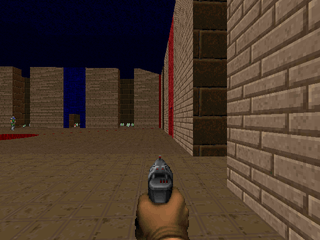
\includegraphics[width=0.23\linewidth]{img/demo_0.png}};
    \node[inner sep=0,right=of f0] (f1) {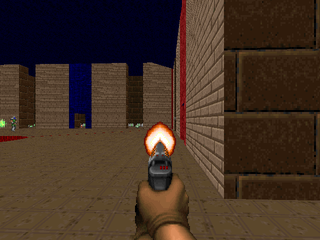
\includegraphics[width=0.23\linewidth]{img/demo_1.png}};
    \node[inner sep=0,right=of f1] (f2) {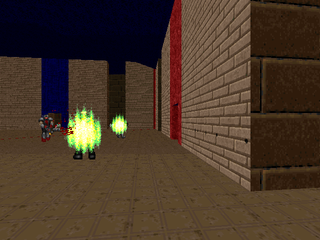
\includegraphics[width=0.23\linewidth]{img/demo_2.png}};
    \node[inner sep=0,right=of f2] (f3) {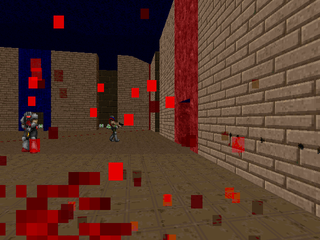
\includegraphics[width=0.23\linewidth]{img/demo_3.png}};
    \foreach \n/\t/\c in {f0/2\,s/start, f1/10\,s/strzał w ścianę, f2/16\,s/atak potworów, f3/19\,s/śmierć} {
      \draw[faint,line width=0.6pt] (\n.south west) rectangle (\n.north east);
      \node[below=1.5mm of \n,font=\scriptsize,align=center]
        {\textbf{\textcolor{accent}{\t}}\\[-0.5mm]\textcolor{muted}{\c}};
    }
  \end{tikzpicture}

  \vspace{3mm}
  \tcbox[colback=accent,colframe=accent,coltext=white,arc=1.5mm,boxsep=1.5mm,left=2mm,right=2mm,top=0.5mm,bottom=0.5mm]
    {\href{run:media/random_agent.mp4}{\small\faPlay\hspace{2mm}\textbf{Odtwórz film} \footnotesize(media/random\_agent.mp4)}}

  \vspace{1mm}
  {\footnotesize\color{muted} Typowy epizod: akcja losowana co 4 klatki, 1 zabójstwo,
  śmierć po 678 tikach (19\,s). Agent losowy to dolny punkt odniesienia.}
\end{frame}

% ============================================================
\renewcommand{\slidenum}{05}
\begin{frame}{Agent losowy -- wyniki}
  \vspace{-2mm}
  \begin{columns}[T,onlytextwidth]
    \begin{column}{0.45\textwidth}
      {\small\textbf{Średnio na epizod}\par}
      {\scriptsize\color{muted}5 seedów $\times$ 100 epizodów, pod wartością 95\% CI\par}
      \vspace{1.5mm}
      \footnotesize
      \renewcommand{\arraystretch}{1.25}
      \begin{tabular}{@{}l>{\raggedleft\arraybackslash}p{0.27\linewidth}>{\raggedleft\arraybackslash}p{0.3\linewidth}@{}}
        & \textcolor{accent}{\rule[0.1ex]{2mm}{2mm}}\hspace{1.5mm}\textbf{strzela}
        & \textcolor{control}{\rule[0.1ex]{2mm}{2mm}}\hspace{1.5mm}\textbf{nie strzela} \\
        \midrule
        Zabójstwa & \begin{tabular}[t]{@{}r@{}}\textbf{1,09}\\[-1mm]{\scriptsize\color{muted}0,96--1,18}\end{tabular} & \begin{tabular}[t]{@{}r@{}}\textbf{0,94}\\[-1mm]{\scriptsize\color{muted}0,89--0,98}\end{tabular} \\[4mm]
        Nagroda & \begin{tabular}[t]{@{}r@{}}\textbf{2,20}\\[-1mm]{\scriptsize\color{muted}1,88--2,50}\end{tabular} & \begin{tabular}[t]{@{}r@{}}\textbf{1,91}\\[-1mm]{\scriptsize\color{muted}1,80--2,03}\end{tabular} \\[4mm]
        Przeżycie & \textbf{17,9\,s} & \textbf{20,4\,s} \\
        Oddane strzały & \textbf{1,7} & \textbf{0} \\
        Śmierć & \textbf{100\%} & \textbf{100\%} \\
        \bottomrule
      \end{tabular}
    \end{column}
    \begin{column}{0.52\textwidth}
      {\small\textbf{Rozkład zabójstw na epizod}\par}
      {\scriptsize\color{muted}odsetek epizodów\par}
      \vspace{1mm}
      \begin{tikzpicture}
        \begin{axis}[
            width=\linewidth, height=4.3cm,
            ybar=0.6pt, bar width=3.6mm,
            ymin=0, ymax=55, ytick={0,25,50},
            yticklabel={\pgfmathprintnumber{\tick}\%},
            yticklabel style={font=\scriptsize,text=muted},
            ymajorgrids, grid style={faint,line width=0.4pt},
            axis x line*=bottom, axis y line*=none, y axis line style={draw=none},
            xtick=data, symbolic x coords={0,1,2,3,4,5,6+},
            xticklabel style={font=\small,text=muted},
            x axis line style={faint},
            major tick length=0pt,
            enlarge x limits=0.09,
            xlabel={liczba zabójstw}, xlabel style={font=\scriptsize,text=muted},
            legend style={draw=none,fill=none,font=\scriptsize,text=ink,at={(1,1.02)},anchor=south east,legend columns=2,/tikz/every even column/.append style={column sep=3mm}},
            square legend,
          ]
          \addplot[fill=accent,draw=none]
            coordinates {(0,47.6) (1,22.8) (2,15.8) (3,7.2) (4,4.0) (5,1.6) (6+,1.0)};
          \addplot[fill=control,draw=none]
            coordinates {(0,51.4) (1,26.0) (2,11.6) (3,5.4) (4,2.6) (5,1.6) (6+,1.4)};
          \legend{strzela, nie strzela}
        \end{axis}
      \end{tikzpicture}
    \end{column}
  \end{columns}

  \vspace{1mm}
  \begin{tcolorbox}[enhanced, colback=accentsoft, colframe=accentsoft, arc=2mm,
      left=3mm, right=3mm, top=1.2mm, bottom=1.2mm, before skip=0pt, after skip=0pt,
      fontupper=\footnotesize]
    \textcolor{accent}{\faExclamationTriangle}\hspace{2mm}Agent, który \textbf{nigdy nie strzela},
    ma \textbf{86\%} zabójstw agenta losowego. Gra liczy też potwory zabite przez
    \textbf{inne potwory}, więc liczba zabójstw i~nagroda zawyżają umiejętności agenta.
  \end{tcolorbox}
\end{frame}

% ============================================================
\renewcommand{\slidenum}{06}
\begin{frame}{Protokół ewaluacji}
  \begin{columns}[T,onlytextwidth]
    \begin{column}{0.48\textwidth}
      \begin{infocard}{\faRedo}{Powtarzalność}
        5 seedów $\times$ 100 epizodów. Ten sam seed ustawia
        politykę agenta i silnik gry, więc każdy przebieg da się odtworzyć.
      \end{infocard}
      \begin{infocard}{\faChartBar}{Statystyki}
        Wynik główny: średnia ze średnich dla seedów $\pm$ odchylenie
        i~95\% przedział ufności (bootstrap). Dodatkowo IQM,
        odporna na pojedyncze rekordowe epizody.
      \end{infocard}
    \end{column}
    \begin{column}{0.48\textwidth}
      {\small\textbf{Metryki na epizod}\par}
      \vspace{2mm}
      \footnotesize
      \renewcommand{\arraystretch}{1.25}
      \begin{tabular}{@{}ll@{}}
        \textcolor{accent}{\faSkull} & zabójstwa, zabójstwa / minutę \\
        \textcolor{accent}{\faHeartbeat} & czas przeżycia, śmierć vs. limit czasu \\
        \textcolor{accent}{\faStar} & suma nagród \\
        \textcolor{accent}{\faBullseye} & oddane strzały, zabójstwa / strzał \\
        \textcolor{accent}{\faShield*} & otrzymane obrażenia i trafienia \\
        \textcolor{accent}{\faBoxOpen} & zebrana amunicja, zdrowie, pancerz \\
        \textcolor{accent}{\faRoute} & przebyta droga \\
        \textcolor{accent}{\faRandom} & entropia wybieranych akcji \\
      \end{tabular}
    \end{column}
  \end{columns}
\end{frame}

% ============================================================
\renewcommand{\slidenum}{07}
\begin{frame}{Plan dalszej pracy}
  \vspace{14mm}
  \begin{tikzpicture}[x=1cm,y=1cm]
    \draw[faint,line width=2pt] (0,0) -- (13.6,0);
    \draw[accent,line width=2pt] (0,0) -- (2.6,0);
    \foreach \x/\done/\head/\body in {
        1.3/1/Pipeline/{wrapper, metryki,\\ewaluacja, testy, CI},
        4.05/0/Preprocessing/{60\,$\times$\,45, stos klatek,\\kształtowanie nagrody},
        6.8/0/Agent DQN/{CNN +\\replay buffer},
        9.55/0/Cel pośredni/{istotnie lepszy\\od agenta losowego},
        12.3/0/Cel końcowy/{skuteczne zabijanie\\i dłuższe przeżycie}} {
      \ifnum\done=1
        \fill[accent] (\x,0) circle (2.2mm);
        \node[text=white,font=\tiny] at (\x,0) {\faCheck};
      \else
        \fill[paper] (\x,0) circle (2.2mm);
        \draw[accent,line width=1pt] (\x,0) circle (2.2mm);
      \fi
      \node[above=4mm,font=\small\bfseries,text=ink] at (\x,0) {\head};
      \node[below=4mm,font=\scriptsize,text=muted,align=center,anchor=north] at (\x,0) {\body};
    }
  \end{tikzpicture}

\end{frame}

\end{document}
